\documentclass[]{article}
\usepackage{lmodern}
\usepackage{amssymb,amsmath}
\usepackage{ifxetex,ifluatex}
\usepackage{fixltx2e} % provides \textsubscript
\ifnum 0\ifxetex 1\fi\ifluatex 1\fi=0 % if pdftex
  \usepackage[T1]{fontenc}
  \usepackage[utf8]{inputenc}
\else % if luatex or xelatex
  \ifxetex
    \usepackage{mathspec}
  \else
    \usepackage{fontspec}
  \fi
  \defaultfontfeatures{Ligatures=TeX,Scale=MatchLowercase}
\fi
% use upquote if available, for straight quotes in verbatim environments
\IfFileExists{upquote.sty}{\usepackage{upquote}}{}
% use microtype if available
\IfFileExists{microtype.sty}{%
\usepackage{microtype}
\UseMicrotypeSet[protrusion]{basicmath} % disable protrusion for tt fonts
}{}
\usepackage[margin=1in]{geometry}
\usepackage{hyperref}
\hypersetup{unicode=true,
            pdftitle={ReproducibleResearch-Project1},
            pdfauthor={Hari Ravichandran},
            pdfborder={0 0 0},
            breaklinks=true}
\urlstyle{same}  % don't use monospace font for urls
\usepackage{color}
\usepackage{fancyvrb}
\newcommand{\VerbBar}{|}
\newcommand{\VERB}{\Verb[commandchars=\\\{\}]}
\DefineVerbatimEnvironment{Highlighting}{Verbatim}{commandchars=\\\{\}}
% Add ',fontsize=\small' for more characters per line
\usepackage{framed}
\definecolor{shadecolor}{RGB}{248,248,248}
\newenvironment{Shaded}{\begin{snugshade}}{\end{snugshade}}
\newcommand{\KeywordTok}[1]{\textcolor[rgb]{0.13,0.29,0.53}{\textbf{#1}}}
\newcommand{\DataTypeTok}[1]{\textcolor[rgb]{0.13,0.29,0.53}{#1}}
\newcommand{\DecValTok}[1]{\textcolor[rgb]{0.00,0.00,0.81}{#1}}
\newcommand{\BaseNTok}[1]{\textcolor[rgb]{0.00,0.00,0.81}{#1}}
\newcommand{\FloatTok}[1]{\textcolor[rgb]{0.00,0.00,0.81}{#1}}
\newcommand{\ConstantTok}[1]{\textcolor[rgb]{0.00,0.00,0.00}{#1}}
\newcommand{\CharTok}[1]{\textcolor[rgb]{0.31,0.60,0.02}{#1}}
\newcommand{\SpecialCharTok}[1]{\textcolor[rgb]{0.00,0.00,0.00}{#1}}
\newcommand{\StringTok}[1]{\textcolor[rgb]{0.31,0.60,0.02}{#1}}
\newcommand{\VerbatimStringTok}[1]{\textcolor[rgb]{0.31,0.60,0.02}{#1}}
\newcommand{\SpecialStringTok}[1]{\textcolor[rgb]{0.31,0.60,0.02}{#1}}
\newcommand{\ImportTok}[1]{#1}
\newcommand{\CommentTok}[1]{\textcolor[rgb]{0.56,0.35,0.01}{\textit{#1}}}
\newcommand{\DocumentationTok}[1]{\textcolor[rgb]{0.56,0.35,0.01}{\textbf{\textit{#1}}}}
\newcommand{\AnnotationTok}[1]{\textcolor[rgb]{0.56,0.35,0.01}{\textbf{\textit{#1}}}}
\newcommand{\CommentVarTok}[1]{\textcolor[rgb]{0.56,0.35,0.01}{\textbf{\textit{#1}}}}
\newcommand{\OtherTok}[1]{\textcolor[rgb]{0.56,0.35,0.01}{#1}}
\newcommand{\FunctionTok}[1]{\textcolor[rgb]{0.00,0.00,0.00}{#1}}
\newcommand{\VariableTok}[1]{\textcolor[rgb]{0.00,0.00,0.00}{#1}}
\newcommand{\ControlFlowTok}[1]{\textcolor[rgb]{0.13,0.29,0.53}{\textbf{#1}}}
\newcommand{\OperatorTok}[1]{\textcolor[rgb]{0.81,0.36,0.00}{\textbf{#1}}}
\newcommand{\BuiltInTok}[1]{#1}
\newcommand{\ExtensionTok}[1]{#1}
\newcommand{\PreprocessorTok}[1]{\textcolor[rgb]{0.56,0.35,0.01}{\textit{#1}}}
\newcommand{\AttributeTok}[1]{\textcolor[rgb]{0.77,0.63,0.00}{#1}}
\newcommand{\RegionMarkerTok}[1]{#1}
\newcommand{\InformationTok}[1]{\textcolor[rgb]{0.56,0.35,0.01}{\textbf{\textit{#1}}}}
\newcommand{\WarningTok}[1]{\textcolor[rgb]{0.56,0.35,0.01}{\textbf{\textit{#1}}}}
\newcommand{\AlertTok}[1]{\textcolor[rgb]{0.94,0.16,0.16}{#1}}
\newcommand{\ErrorTok}[1]{\textcolor[rgb]{0.64,0.00,0.00}{\textbf{#1}}}
\newcommand{\NormalTok}[1]{#1}
\usepackage{graphicx,grffile}
\makeatletter
\def\maxwidth{\ifdim\Gin@nat@width>\linewidth\linewidth\else\Gin@nat@width\fi}
\def\maxheight{\ifdim\Gin@nat@height>\textheight\textheight\else\Gin@nat@height\fi}
\makeatother
% Scale images if necessary, so that they will not overflow the page
% margins by default, and it is still possible to overwrite the defaults
% using explicit options in \includegraphics[width, height, ...]{}
\setkeys{Gin}{width=\maxwidth,height=\maxheight,keepaspectratio}
\IfFileExists{parskip.sty}{%
\usepackage{parskip}
}{% else
\setlength{\parindent}{0pt}
\setlength{\parskip}{6pt plus 2pt minus 1pt}
}
\setlength{\emergencystretch}{3em}  % prevent overfull lines
\providecommand{\tightlist}{%
  \setlength{\itemsep}{0pt}\setlength{\parskip}{0pt}}
\setcounter{secnumdepth}{0}
% Redefines (sub)paragraphs to behave more like sections
\ifx\paragraph\undefined\else
\let\oldparagraph\paragraph
\renewcommand{\paragraph}[1]{\oldparagraph{#1}\mbox{}}
\fi
\ifx\subparagraph\undefined\else
\let\oldsubparagraph\subparagraph
\renewcommand{\subparagraph}[1]{\oldsubparagraph{#1}\mbox{}}
\fi

%%% Use protect on footnotes to avoid problems with footnotes in titles
\let\rmarkdownfootnote\footnote%
\def\footnote{\protect\rmarkdownfootnote}

%%% Change title format to be more compact
\usepackage{titling}

% Create subtitle command for use in maketitle
\newcommand{\subtitle}[1]{
  \posttitle{
    \begin{center}\large#1\end{center}
    }
}

\setlength{\droptitle}{-2em}
  \title{ReproducibleResearch-Project1}
  \pretitle{\vspace{\droptitle}\centering\huge}
  \posttitle{\par}
  \author{Hari Ravichandran}
  \preauthor{\centering\large\emph}
  \postauthor{\par}
  \predate{\centering\large\emph}
  \postdate{\par}
  \date{May 4, 2018}


\begin{document}
\maketitle

\section{Libraries}\label{libraries}

\begin{Shaded}
\begin{Highlighting}[]
\KeywordTok{library}\NormalTok{(lubridate) }\CommentTok{#For date conversion}
\end{Highlighting}
\end{Shaded}

\begin{verbatim}
## Warning: package 'lubridate' was built under R version 3.4.4
\end{verbatim}

\begin{verbatim}
## 
## Attaching package: 'lubridate'
\end{verbatim}

\begin{verbatim}
## The following object is masked from 'package:base':
## 
##     date
\end{verbatim}

\begin{Shaded}
\begin{Highlighting}[]
\KeywordTok{library}\NormalTok{(ggplot2) }\CommentTok{#For Plotting}
\end{Highlighting}
\end{Shaded}

\begin{verbatim}
## Warning: package 'ggplot2' was built under R version 3.4.4
\end{verbatim}

\begin{Shaded}
\begin{Highlighting}[]
\KeywordTok{library}\NormalTok{(gridExtra) }\CommentTok{#For qplot() -> grid.arrange()}
\end{Highlighting}
\end{Shaded}

\begin{verbatim}
## Warning: package 'gridExtra' was built under R version 3.4.4
\end{verbatim}

\section{Load the Data}\label{load-the-data}

\begin{Shaded}
\begin{Highlighting}[]
\NormalTok{S <-}\StringTok{ }\KeywordTok{read.csv}\NormalTok{(}\StringTok{"activity.csv"}\NormalTok{) }\CommentTok{#Loads data into data frame}
\NormalTok{S}\OperatorTok{$}\NormalTok{date <-}\StringTok{ }\KeywordTok{ymd}\NormalTok{(S}\OperatorTok{$}\NormalTok{date) }\CommentTok{#Convert 'date' column from factor to date}
\KeywordTok{class}\NormalTok{(S}\OperatorTok{$}\NormalTok{date) }\CommentTok{#Check class of S$date}
\end{Highlighting}
\end{Shaded}

\begin{verbatim}
## [1] "Date"
\end{verbatim}

\begin{Shaded}
\begin{Highlighting}[]
\NormalTok{S1 <-}\StringTok{ }\KeywordTok{na.omit}\NormalTok{(S) }\CommentTok{#Remove all NA values}
\KeywordTok{head}\NormalTok{(S1) }\CommentTok{#Print out S1}
\end{Highlighting}
\end{Shaded}

\begin{verbatim}
##     steps       date interval
## 289     0 2012-10-02        0
## 290     0 2012-10-02        5
## 291     0 2012-10-02       10
## 292     0 2012-10-02       15
## 293     0 2012-10-02       20
## 294     0 2012-10-02       25
\end{verbatim}

\section{Make Histogram of Daily
Data}\label{make-histogram-of-daily-data}

\begin{Shaded}
\begin{Highlighting}[]
\NormalTok{S_sum <-}\StringTok{ }\KeywordTok{aggregate}\NormalTok{(steps}\OperatorTok{~}\NormalTok{date, S1, sum) }\CommentTok{#Total Steps taken per day}
\KeywordTok{head}\NormalTok{(S_sum)}
\end{Highlighting}
\end{Shaded}

\begin{verbatim}
##         date steps
## 1 2012-10-02   126
## 2 2012-10-03 11352
## 3 2012-10-04 12116
## 4 2012-10-05 13294
## 5 2012-10-06 15420
## 6 2012-10-07 11015
\end{verbatim}

\begin{Shaded}
\begin{Highlighting}[]
\CommentTok{#Histogram of total steps taken each day}
\KeywordTok{qplot}\NormalTok{(steps, }\DataTypeTok{data =}\NormalTok{ S_sum , }\DataTypeTok{geom =} \StringTok{"histogram"}\NormalTok{, }\DataTypeTok{binwidth =} \DecValTok{500}\NormalTok{, }\DataTypeTok{fill =} \StringTok{"red"}\NormalTok{) }\OperatorTok{+}\StringTok{ }
\StringTok{    }\KeywordTok{labs}\NormalTok{(}\DataTypeTok{title =} \StringTok{"Total Number of Steps Each Day"}\NormalTok{, }\DataTypeTok{x =} \StringTok{"Number of Steps"}\NormalTok{, }\DataTypeTok{y =} \StringTok{"Frequency"}\NormalTok{)}
\end{Highlighting}
\end{Shaded}

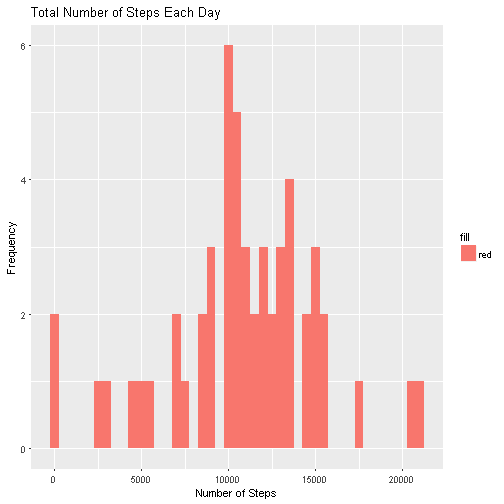
\includegraphics{PA1_template_files/figure-latex/histogram-1.pdf}

\subsection{Compute Mean and Median}\label{compute-mean-and-median}

\begin{Shaded}
\begin{Highlighting}[]
\NormalTok{mean_daily <-}\StringTok{ }\KeywordTok{mean}\NormalTok{(S_sum}\OperatorTok{$}\NormalTok{steps) }\CommentTok{#Mean of total number of steps}
\KeywordTok{print}\NormalTok{(mean_daily)}
\end{Highlighting}
\end{Shaded}

\begin{verbatim}
## [1] 10766.19
\end{verbatim}

\begin{Shaded}
\begin{Highlighting}[]
\NormalTok{median_daily <-}\StringTok{ }\KeywordTok{median}\NormalTok{(S_sum}\OperatorTok{$}\NormalTok{steps) }\CommentTok{#Mdian of total number of steps}
\KeywordTok{print}\NormalTok{(median_daily)}
\end{Highlighting}
\end{Shaded}

\begin{verbatim}
## [1] 10765
\end{verbatim}

\section{Make Time-Series Plot Based on
Intervals}\label{make-time-series-plot-based-on-intervals}

\begin{Shaded}
\begin{Highlighting}[]
\NormalTok{S_intervals <-}\StringTok{ }\KeywordTok{aggregate}\NormalTok{(steps}\OperatorTok{~}\NormalTok{interval, S1, sum) }\CommentTok{#Sum up values at each interval}
\KeywordTok{head}\NormalTok{(S_intervals)}
\end{Highlighting}
\end{Shaded}

\begin{verbatim}
##   interval steps
## 1        0    91
## 2        5    18
## 3       10     7
## 4       15     8
## 5       20     4
## 6       25   111
\end{verbatim}

\begin{Shaded}
\begin{Highlighting}[]
\KeywordTok{plot}\NormalTok{(S_intervals}\OperatorTok{$}\NormalTok{interval, S_intervals}\OperatorTok{$}\NormalTok{steps, }\DataTypeTok{type =} \StringTok{"l"}\NormalTok{) }\CommentTok{#Make time-series plot}
\end{Highlighting}
\end{Shaded}

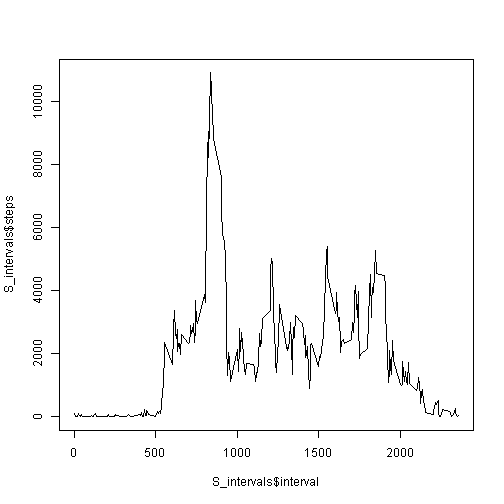
\includegraphics{PA1_template_files/figure-latex/intervals-1.pdf}

\begin{Shaded}
\begin{Highlighting}[]
\NormalTok{max_ind <-}\StringTok{ }\KeywordTok{which.max}\NormalTok{(S_intervals}\OperatorTok{$}\NormalTok{steps) }\CommentTok{#Find & print the max interval with the most steps}
\NormalTok{max_interval <-}\StringTok{ }\NormalTok{S}\OperatorTok{$}\NormalTok{interval[max_ind]}
\KeywordTok{print}\NormalTok{(max_interval)}
\end{Highlighting}
\end{Shaded}

\begin{verbatim}
## [1] 835
\end{verbatim}

\section{Total Number of NA Values in Data
Set}\label{total-number-of-na-values-in-data-set}

\begin{Shaded}
\begin{Highlighting}[]
\KeywordTok{print}\NormalTok{(}\KeywordTok{sum}\NormalTok{(}\KeywordTok{is.na}\NormalTok{(S)))}
\end{Highlighting}
\end{Shaded}

\begin{verbatim}
## [1] 2304
\end{verbatim}

\subsection{Fill in NA Values with Zeros for 5 Minute
Interval}\label{fill-in-na-values-with-zeros-for-5-minute-interval}

\begin{Shaded}
\begin{Highlighting}[]
\NormalTok{S_fill <-}\StringTok{ }\NormalTok{S}
\NormalTok{S_fill[}\KeywordTok{is.na}\NormalTok{(S_fill)] <-}\StringTok{ }\DecValTok{0} \CommentTok{#We fill in the NA values with zero}

\KeywordTok{head}\NormalTok{(S_fill)}
\end{Highlighting}
\end{Shaded}

\begin{verbatim}
##   steps       date interval
## 1     0 2012-10-01        0
## 2     0 2012-10-01        5
## 3     0 2012-10-01       10
## 4     0 2012-10-01       15
## 5     0 2012-10-01       20
## 6     0 2012-10-01       25
\end{verbatim}

\section{Make Histogram of Daily Data for Filled
Data}\label{make-histogram-of-daily-data-for-filled-data}

\begin{Shaded}
\begin{Highlighting}[]
\NormalTok{S_sum_fill <-}\StringTok{ }\KeywordTok{aggregate}\NormalTok{(steps}\OperatorTok{~}\NormalTok{date, S_fill, sum) }\CommentTok{#Use aggregate to sum up values at each time --> daily}
\KeywordTok{head}\NormalTok{(S_sum_fill)}
\end{Highlighting}
\end{Shaded}

\begin{verbatim}
##         date steps
## 1 2012-10-01     0
## 2 2012-10-02   126
## 3 2012-10-03 11352
## 4 2012-10-04 12116
## 5 2012-10-05 13294
## 6 2012-10-06 15420
\end{verbatim}

\begin{Shaded}
\begin{Highlighting}[]
\CommentTok{#Plot Histogram}
\KeywordTok{qplot}\NormalTok{(steps, }\DataTypeTok{data =}\NormalTok{ S_sum_fill , }\DataTypeTok{geom =} \StringTok{"histogram"}\NormalTok{, }\DataTypeTok{binwidth =} \DecValTok{500}\NormalTok{, }\DataTypeTok{fill =} \StringTok{"red"}\NormalTok{)  }\OperatorTok{+}\StringTok{ }
\StringTok{    }\KeywordTok{labs}\NormalTok{(}\DataTypeTok{title =} \StringTok{"Total Number of Steps Each Day"}\NormalTok{, }\DataTypeTok{x =} \StringTok{"Number of Steps"}\NormalTok{, }\DataTypeTok{y =} \StringTok{"Frequency"}\NormalTok{)}
\end{Highlighting}
\end{Shaded}

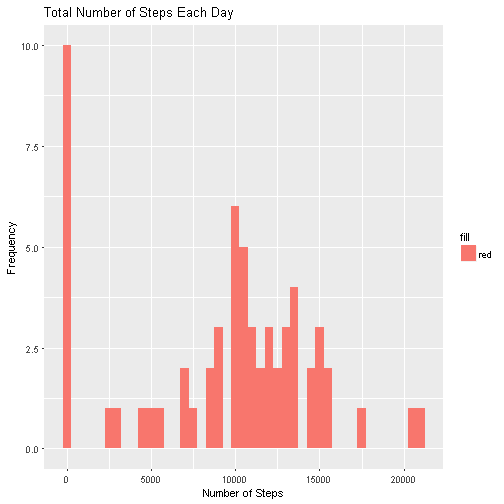
\includegraphics{PA1_template_files/figure-latex/histogram-fill-1.pdf}

\subsection{Compute Mean and Median for Filled
Data}\label{compute-mean-and-median-for-filled-data}

\begin{Shaded}
\begin{Highlighting}[]
\NormalTok{mean_daily_fill <-}\StringTok{ }\KeywordTok{mean}\NormalTok{(S_sum_fill}\OperatorTok{$}\NormalTok{steps)  }\CommentTok{#Mean of total number of steps}
\KeywordTok{print}\NormalTok{(mean_daily_fill)}
\end{Highlighting}
\end{Shaded}

\begin{verbatim}
## [1] 9354.23
\end{verbatim}

\begin{Shaded}
\begin{Highlighting}[]
\NormalTok{median_daily_fill <-}\StringTok{ }\KeywordTok{median}\NormalTok{(S_sum_fill}\OperatorTok{$}\NormalTok{steps)  }\CommentTok{#Median of total number of steps}
\KeywordTok{print}\NormalTok{(median_daily_fill)}
\end{Highlighting}
\end{Shaded}

\begin{verbatim}
## [1] 10395
\end{verbatim}

\section{Differences between Weekdays and
Weekends?}\label{differences-between-weekdays-and-weekends}

\begin{Shaded}
\begin{Highlighting}[]
\NormalTok{W <-}\StringTok{ }\KeywordTok{wday}\NormalTok{(S_fill}\OperatorTok{$}\NormalTok{date) }\CommentTok{#Use lubridate wday()}
\NormalTok{Is_Weekday <-}\StringTok{ }\KeywordTok{ifelse}\NormalTok{(W }\OperatorTok\StringTok{ }\KeywordTok{c}\NormalTok{(}\DecValTok{2}\NormalTok{,}\DecValTok{3}\NormalTok{,}\DecValTok{4}\NormalTok{,}\DecValTok{5}\NormalTok{,}\DecValTok{6}\NormalTok{), }\StringTok{"Weekday"}\NormalTok{, }\StringTok{"Weekend"}\NormalTok{) }\CommentTok{#2 - 6 are Mon - Fri}

\NormalTok{S_fill}\OperatorTok{$}\NormalTok{Is_Weekday <-}\StringTok{ }\KeywordTok{factor}\NormalTok{(Is_Weekday) }\CommentTok{#Create the factor variable for weekdays/weekends}

\KeywordTok{head}\NormalTok{(S_fill)}
\end{Highlighting}
\end{Shaded}

\begin{verbatim}
##   steps       date interval Is_Weekday
## 1     0 2012-10-01        0    Weekday
## 2     0 2012-10-01        5    Weekday
## 3     0 2012-10-01       10    Weekday
## 4     0 2012-10-01       15    Weekday
## 5     0 2012-10-01       20    Weekday
## 6     0 2012-10-01       25    Weekday
\end{verbatim}

\subsection{Panel Plot with Time Series Plot for
Weekdays/Weekends}\label{panel-plot-with-time-series-plot-for-weekdaysweekends}

\begin{Shaded}
\begin{Highlighting}[]
\NormalTok{split_wdays <-}\StringTok{ }\KeywordTok{split}\NormalTok{(S_fill, S_fill}\OperatorTok{$}\NormalTok{Is_Weekday)}

\NormalTok{wdays <-}\StringTok{ }\KeywordTok{aggregate}\NormalTok{(steps}\OperatorTok{~}\NormalTok{interval, split_wdays}\OperatorTok{$}\NormalTok{Weekday, sum)}
\NormalTok{wknds <-}\StringTok{ }\KeywordTok{aggregate}\NormalTok{(steps}\OperatorTok{~}\NormalTok{interval, split_wdays}\OperatorTok{$}\NormalTok{Weekend, sum)}

\NormalTok{q_wdays <-}\StringTok{ }\KeywordTok{qplot}\NormalTok{(}\DataTypeTok{x =}\NormalTok{ interval, }\DataTypeTok{y =}\NormalTok{ steps, }\DataTypeTok{data =}\NormalTok{ wdays, }\DataTypeTok{geom =} \StringTok{"line"}\NormalTok{) }\OperatorTok{+}\StringTok{ }\KeywordTok{ggtitle}\NormalTok{(}\StringTok{"Weekdays"}\NormalTok{)}
\NormalTok{q_wknds <-}\StringTok{ }\KeywordTok{qplot}\NormalTok{(}\DataTypeTok{x =}\NormalTok{ interval, }\DataTypeTok{y =}\NormalTok{ steps, }\DataTypeTok{data =}\NormalTok{ wknds, }\DataTypeTok{geom =} \StringTok{"line"}\NormalTok{) }\OperatorTok{+}\StringTok{ }\KeywordTok{ggtitle}\NormalTok{(}\StringTok{"Weekends"}\NormalTok{)}

\KeywordTok{grid.arrange}\NormalTok{(q_wdays, q_wknds, }\DataTypeTok{ncol =} \DecValTok{1}\NormalTok{)}
\end{Highlighting}
\end{Shaded}

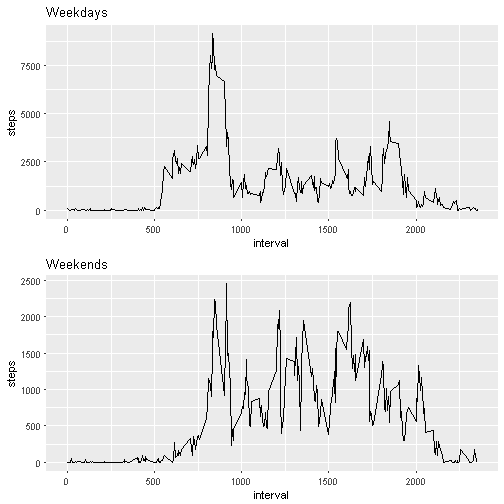
\includegraphics{PA1_template_files/figure-latex/timeseries-weekdays-1.pdf}


\end{document}
